\documentclass{beamer}
\usepackage{../../shared/styles/custom}
\usepackage{../../shared/styles/conventions}

\def\checkmark{\tikz\fill[scale=0.4](0,.35) -- (.25,0) -- (1,.7) -- (.25,.15) -- cycle;} 

%\beamerdefaultoverlayspecification{<+->}




\title{Ridge Regression}
\date{\today}
\author{Nipun Batra}
\institute{IIT Gandhinagar}
\begin{document}
  \maketitle

\begin{frame}{Introduction}
A known measure of overfitting can be the magnitude of the coefficient. \\ \bigskip
\pause
In $f(x) = c_0 + c_1x + c_2x^2 + \dots$ it is $\max|c_i|$ \\ \bigskip
\end{frame}
  
\begin{frame}{Introduction}
\vspace{0.4cm}
\only<1>{\begin{figure}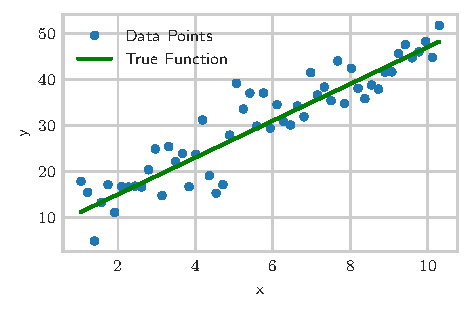
\includegraphics[width=0.8\linewidth]{../assets/ridge-regression/figures/lin_1.pdf}\caption{Base Data Set}
\end{figure}}
\only<2>{\begin{figure}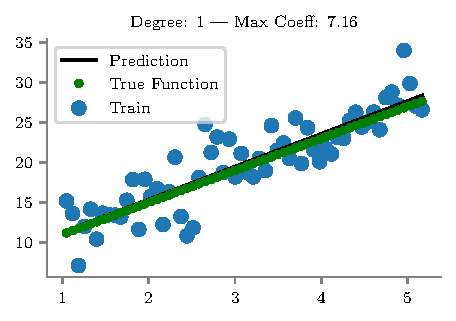
\includegraphics[width=0.8\linewidth]{../assets/ridge-regression/figures/lin_plot_1.pdf}\caption{Fit with Degree 1}
\end{figure}}
\only<3>{\begin{figure}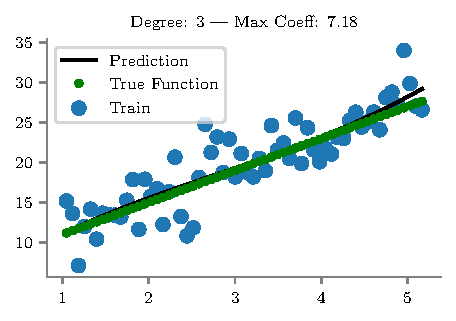
\includegraphics[width=0.8\linewidth]{../assets/ridge-regression/figures/lin_plot_3.pdf}\caption{Fit with Degree 3}
\end{figure}}
\only<4>{\begin{figure}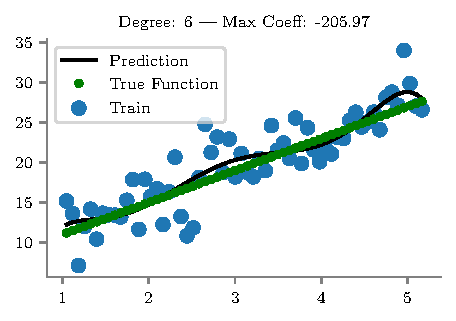
\includegraphics[width=0.8\linewidth]{../assets/ridge-regression/figures/lin_plot_6.pdf}\caption{Fit with Degree 6}
\end{figure}}
\only<5>{\begin{figure}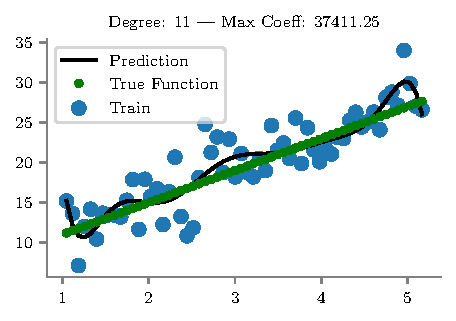
\includegraphics[width=0.8\linewidth]{../assets/ridge-regression/figures/lin_plot_11.pdf}\caption{Fit with Degree 11}
\end{figure}}
\end{frame}  

\begin{frame}{Introduction}
\vspace{0.4cm}
In the examples we notice that as the degree increases (as the prediction starts to overfit the base data), the maximum coefficient also increases.
%\vspace{-0.3cm}
\begin{figure}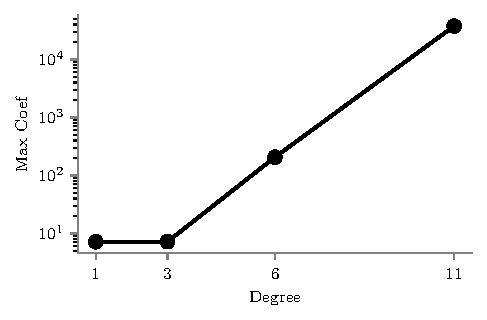
\includegraphics[width=0.7\linewidth]{../assets/ridge-regression/figures/lin_plot_coef.pdf}\caption{Trend of the coefficients}\end{figure}

\end{frame}
 
\begin{frame}{Introduction}
\vspace{0.4cm}
To prevent overfitting we place penalties on large $\theta_i$
\pause
 \\ \bigskip
\begin{tcolorbox}
\textbf{Objective:}
\begin{align*}
\text{Minimise } & \left(\vy-\mX\vtheta\right)^T\left(\vy-\mX\vtheta\right) \\
\text{s.t. } & \vtheta ^T\vtheta \leq S
\end{align*}
\end{tcolorbox}
\pause
This is equivalent to \vspace{-0.4cm}
$$
\text{Minimise } \left(\vy-\mX\vtheta\right)^T\left(\vy-\mX\vtheta\right) + \delta ^2\vtheta ^T\vtheta
$$
\end{frame}  

\begin{frame}{Introduction}
\begin{figure}
        \begin{subfigure}[b]{0.5\textwidth}
                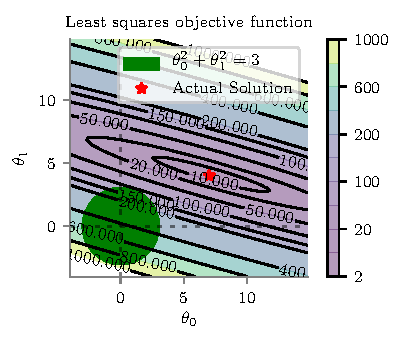
\includegraphics[width=\linewidth]{../assets/ridge-regression/figures/ridge_base_contour.pdf}
                \caption{Contour Plot}
        \end{subfigure}%
        \begin{subfigure}[b]{0.5\textwidth}
                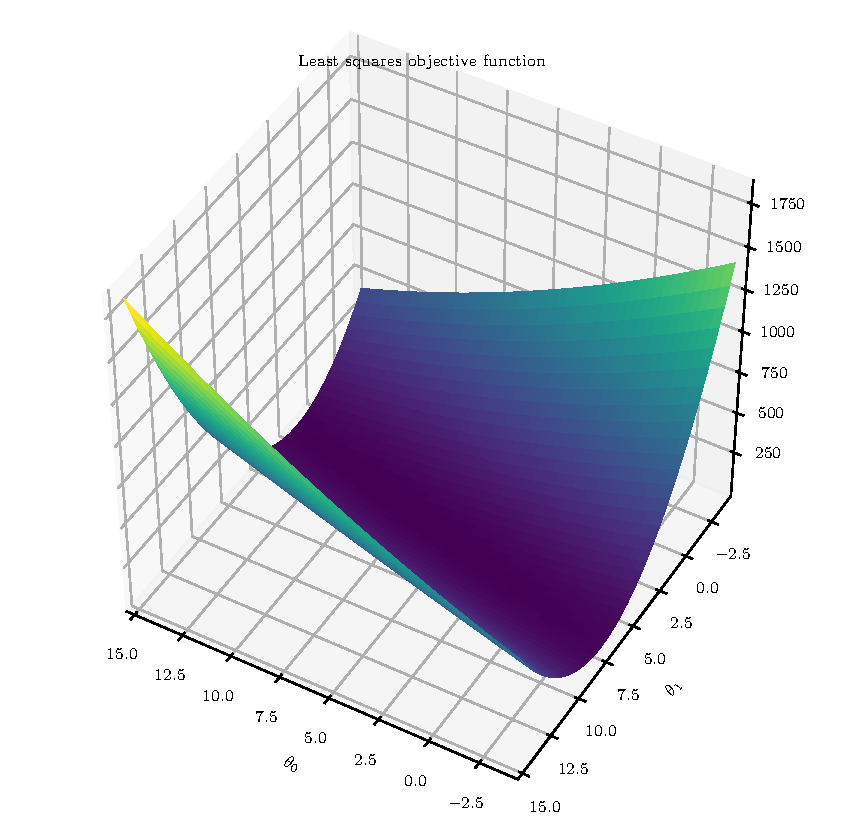
\includegraphics[width=\linewidth]{../assets/ridge-regression/figures/ridge_base_surface.pdf}
                \caption{Surface Plot}
        \end{subfigure}%
        \caption{Visualization of the Example}
\end{figure}
\end{frame}

\begin{frame}{KKT Conditions}
To implement this we use KKT Conditions
\pause
\begin{align*}
\text{Minimise } & \left(\vy-\mX\vtheta\right)^T\left(\vy-\mX\vtheta\right) \\
\text{s.t. } & \vtheta ^T\vtheta \leq S \\
L\left(\vtheta, \mu \right) =& \left(\vy-\mX\vtheta\right)^T\left(\vy-\mX\vtheta\right) + \mu\left(\vtheta^T\vtheta - S\right)
\end{align*}
where, $\mu \geq 0$ (and $\mu = \delta^2$)\bigskip

\pause
\begin{columns}
\begin{column}{0.4\textwidth}
If $\mu = 0$ \\
There is no regularization \\
No effect on constraint
\end{column}
\pause
\begin{column}{0.4\textwidth}
If $\mu\neq 0$ \\
$\implies \vtheta^T\vtheta - S = 0$ 
\end{column}
\end{columns}
\end{frame}

\begin{frame}{Effect of $\mu$}
\vspace{0.4cm}
\only<1>{\begin{figure}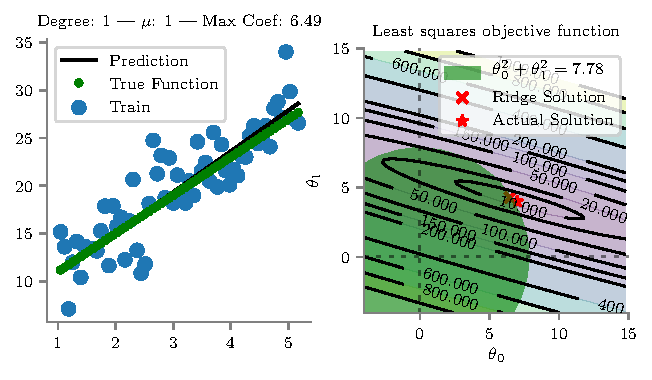
\includegraphics[width=0.8\linewidth]{../assets/ridge-regression/figures/ridge_1.pdf}\caption{$\mu = 1$}
\end{figure}}
\only<2>{\begin{figure}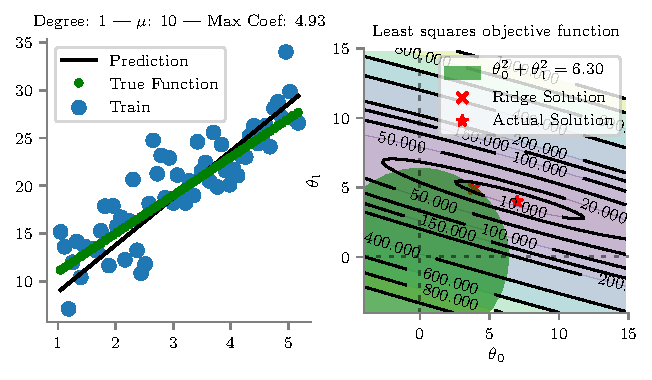
\includegraphics[width=0.8\linewidth]{../assets/ridge-regression/figures/ridge_10.pdf}\caption{$\mu = 10$}
\end{figure}}
\only<3>{\begin{figure}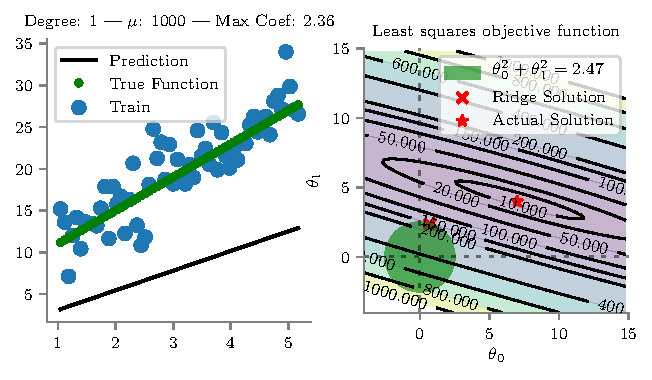
\includegraphics[width=0.8\linewidth]{../assets/ridge-regression/figures/ridge_1000.pdf}\caption{$\mu = 1000$}
\end{figure}}
\end{frame}

%\begin{frame}{Effect of $\mu$ on higher degree fits}
%\vspace{0.4cm}
%\only<1>{\begin{figure}\includegraphics[width=0.8\linewidth]{ridge/ridge_1_16.pdf}\caption{$\mu = 1$ when Degree $= 16$}
%\end{figure}}
%\only<2>{\begin{figure}\includegraphics[width=0.8\linewidth]{ridge/ridge_100_16.pdf}\caption{$\mu = 100$  when Degree $= 16$}
%\end{figure}}
%\only<3>{\begin{figure}\includegraphics[width=0.8\linewidth]{ridge/ridge_100000_16.pdf}\caption{$\mu = 100000$  when Degree $= 16$}
%\end{figure}}
%\end{frame}

\begin{frame}{Effect of $\mu$ - Regularization of Parameters}
\vspace{0.4cm}
\begin{figure}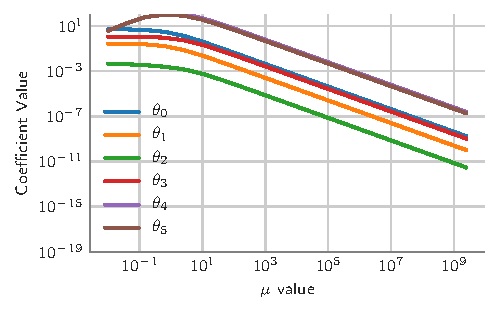
\includegraphics[width=0.8\linewidth]{../assets/ridge-regression/figures/rid_reg-without-lim.pdf}\caption{Comparing the magnitudes of the coefficients with varying $\mu$\\(on the \emph{Real Estate Data Set})}
\end{figure}
\pause Are $\theta_{i}$ all zero for high $\mu$?
\end{frame}

\begin{frame}{Effect of $\mu$ - Regularization of Parameters}
\vspace{0.4cm}
\begin{figure}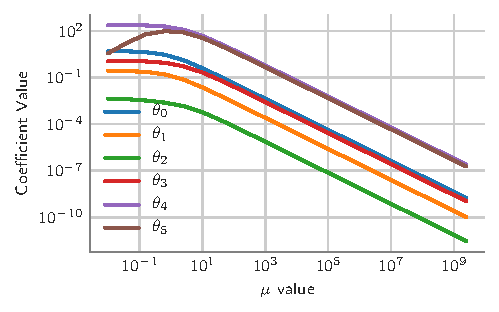
\includegraphics[width=0.8\linewidth]{../assets/ridge-regression/figures/rid_reg-with-lim.pdf}\caption{Comparing the magnitudes of the coefficients with varying $\mu$\\(on the \emph{Real Estate Data Set})}
\end{figure}
\end{frame}

\begin{frame}{Analytical Method}
\begin{tcolorbox}
\textbf{Ridge Objective:}
\vspace{-0.4cm}
$$
\min_{\vtheta} \left(\vy-\mX\vtheta\right)^T\left(\vy-\mX\vtheta\right)+ \mu\vtheta^T\vtheta
$$
\end{tcolorbox}
\begin{align*}
\frac{\partial L\left(\vtheta, \mu\right)}{\partial \vtheta} &= 0 \\ 
\frac{\partial}{\partial \vtheta}\left\lbrace \vy^T\vy - 2\vy^T\mX\vtheta + \vtheta^T\mX^T\mX\vtheta \right\rbrace +  \frac{\partial}{\partial \vtheta} \mu\vtheta^T\vtheta &= 0 \\
\implies -\mX^T\vy + \left(\mX^T\mX + \mu \mI\right)\vtheta &= 0 \\
\implies \vtheta^* &= \left(\mX^T\mX + \mu \mI\right)^{-1}\mX^T\vy
\end{align*}
\end{frame}

\begin{frame}{Bias/Variance}
\begin{columns}
\begin{column}{0.4\textwidth}
\begin{figure}
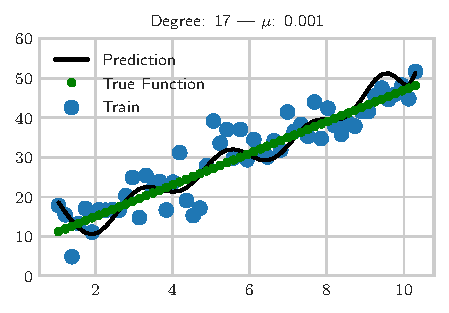
\includegraphics[width=\linewidth]{../assets/ridge-regression/figures/ridge_new_0_17.pdf}
\end{figure}
Fit High Order Polynomial \\
$\implies$ high variance \\
$\implies \, \mu \rightarrow 0$
\end{column}
\begin{column}{0.4\textwidth}
\begin{figure}
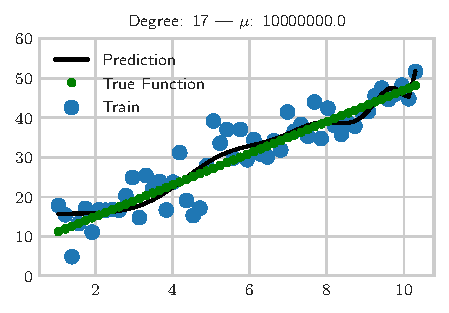
\includegraphics[width=\linewidth]{../assets/ridge-regression/figures/ridge_new_1_17.pdf}
\end{figure}
Fit High Order Polynomial \\
$\implies$ low variance \\
$\implies \, \mu \rightarrow \infty$
\end{column}
\end{columns}
\end{frame}

\begin{frame}{Example}
\vspace{0.4cm}
\textbf{Q.)} Solve Regularized ($\mu = 2$) and Unregularized.
\vspace{-0.6cm}
\begin{figure}
%\includegraphics[width=\linewidth]{../assets/ridge-regression/figures/temp.pdf} % File missing
\end{figure}
\end{frame}

\begin{frame}{Example: Unregularised}
\[
\vtheta = (\mX^{T}\mX)^{-1}(\mX^{T}\vy)
\]
\pause
\begin{align*}
\mX^{T}\mX &= \begin{bmatrix}
4 &10\\10&30
\end{bmatrix} \\
(\mX^{T}\mX)^{-1} &= \frac{1}{20} \begin{bmatrix}
30 & -10\\
-10& 4
\end{bmatrix}\\
\mX^{T}\vy &= \begin{bmatrix}
6\\
14
\end{bmatrix}
\end{align*}
\end{frame}


\begin{frame}{Example: Unregularised}
\vspace{0.4cm}
\begin{align*}
\begin{split}
\vtheta &= (\mX^{T}\mX)^{-1}(\mX^{T}\vy)\\
\begin{bmatrix}
\theta_{0}\\
\theta_{1}
\end{bmatrix} &= 
\begin{bmatrix}
2\\
(-1/5)
\end{bmatrix} 
\end{split}
\end{align*}
\vspace{-0.8cm}
\begin{figure}
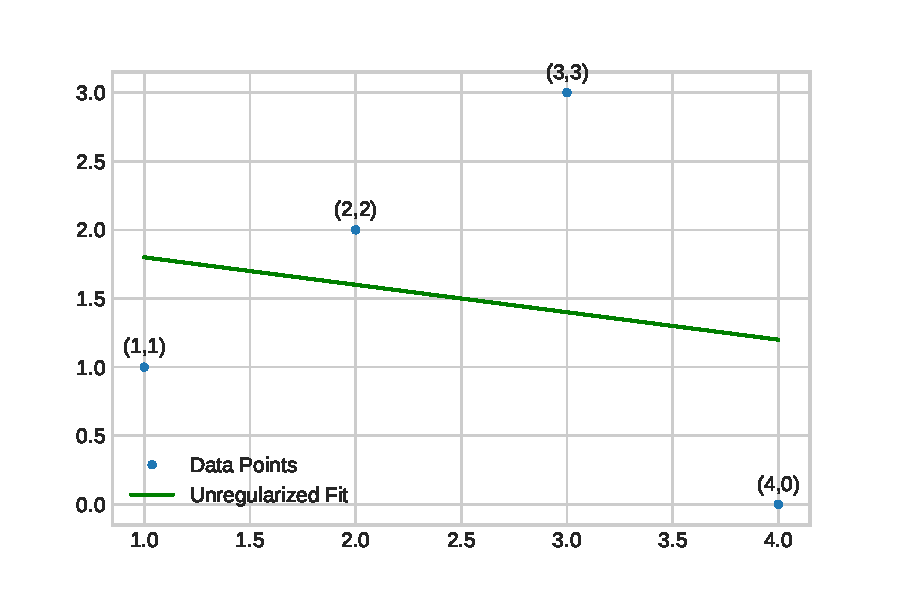
\includegraphics[width=0.8\linewidth]{../assets/ridge-regression/figures/q_unreg.pdf}
\end{figure}
\end{frame}

\begin{frame}{Example: Regularised}
\[
\vtheta = (\mX^{T}\mX+\mu \mI)^{-1}(\mX^{T}\vy)
\]
\pause
\begin{align*}
\mX^{T}\mX &= \begin{bmatrix}
4 &10\\10&30
\end{bmatrix} \\
\mX^{T}\mX+\mu \mI &= \begin{bmatrix}
6 &10\\10&32
\end{bmatrix} \\
(\mX^{T}\mX+\mu \mI)^{-1} &= \frac{1}{92} \begin{bmatrix}
32 & -10\\
-10& 6
\end{bmatrix}\\
\mX^{T}\vy &= \begin{bmatrix}
6\\
14
\end{bmatrix}
\end{align*}
\end{frame}

\begin{frame}{Example: Regularised}
\vspace{0.4cm}
\begin{align*}
\begin{split}
\vtheta &= (\mX^{T}\mX+\mu \mI)^{-1}(\mX^{T}\vy) \\
\begin{bmatrix}
\theta_{0}\\
\theta_{1}
\end{bmatrix} &= 
\begin{bmatrix}
0.56\\
0.26
\end{bmatrix} 
\end{split}
\end{align*}
\vspace{-0.8cm}
\begin{figure}
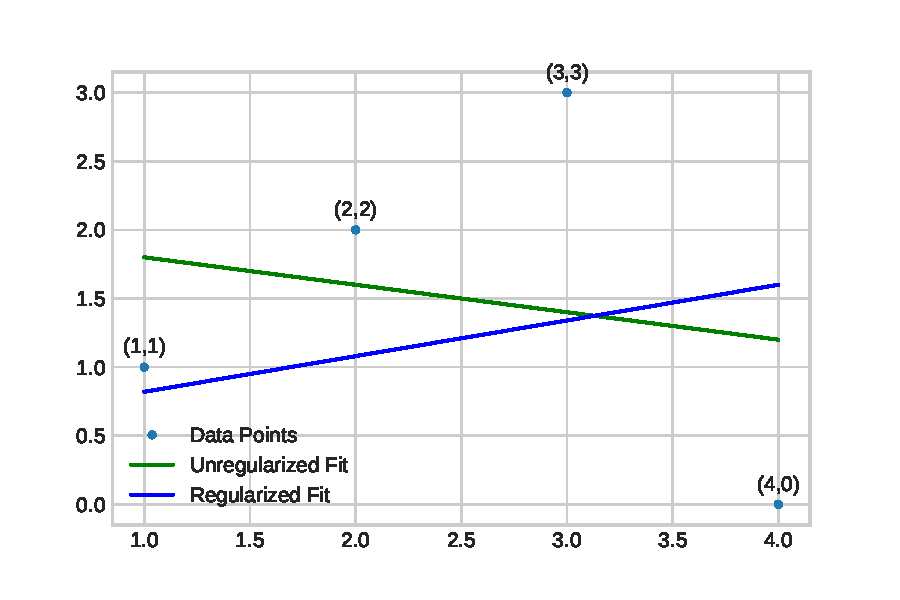
\includegraphics[width=0.8\linewidth]{../assets/ridge-regression/figures/q_reg.pdf}
\end{figure}
\end{frame}

\begin{frame}{Multi-collinearity}
$(\mX^{T}\mX)^{-1}$ is not computable when $|\mX^{T}\mX|$ = 0.

This was a drawback of using linear regression

\begin{equation*}
\mX = \begin{bmatrix}
1 & 1& 2\\
1 & 2& 4\\
1 & 3& 6\\
\end{bmatrix}
\end{equation*}

The matrix $\mX$ is not full rank. 
\end{frame}

\begin{frame}{Multi-collinearity}
But with ridge regression, the matrix to be inverted is $\mX^{T}\mX + \mu \mI$ and not $\mX^{T}\mX$.

\begin{equation*}
\mX^T\mX + \mu \mI = \begin{bmatrix}
3+\mu & 6& 12\\
6 & 14+\mu & 28\\
12 & 28& 56+\mu \\
\end{bmatrix}
\end{equation*}

The matrix $\mX^T\mX$ would be full rank for $\mu>0$. 

\pause Another interpretation of ``regularisation''
\end{frame}


\begin{frame}{Extension of the analytical model}
For ridge with no penalty on $\theta_0$
$$
\hat{\vtheta} = \left(\mX^T\mX+\mu \mI^*\right)^{-1}\mX^T\vy
$$
where, $$\mI^* = \begin{bmatrix}
    \color{red}0 & 0 & 0 & \dots  & 0 \\
    0 & 1& 0 & \dots  & 0\\
    \vdots & \vdots & \vdots & \ddots & \vdots \\
    0 & 0 & 0 & \dots  & 1
\end{bmatrix}$$
\end{frame}


%{
%	\setbeamercolor{background canvas}{bg=}
%	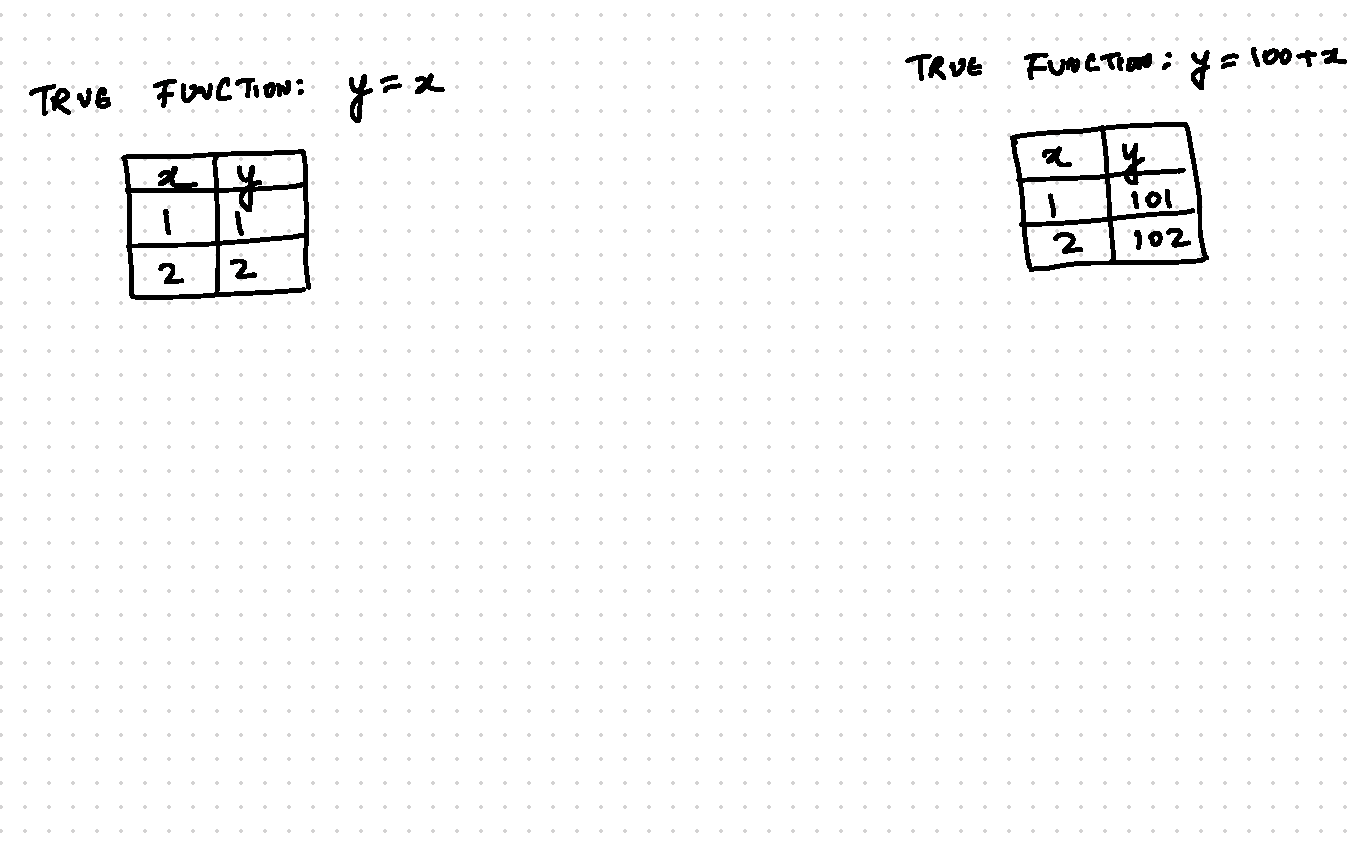
\includepdf[page=-]{ridge-intercept.pdf}
%}


%{
%	\setbeamercolor{background canvas}{bg=}
%	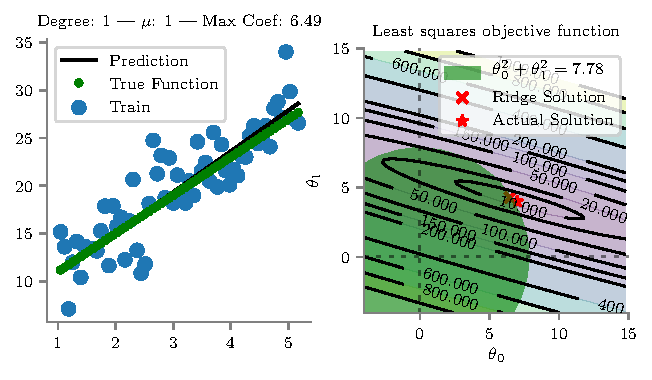
\includepdf[page=-]{ridge-cv.pdf}
%}

\begin{frame}{Ridge Solution using Gradient Descent}
\begin{itemize}[<+->]
	\item \(\vtheta=\vtheta - \alpha \frac{\partial}{\partial \vtheta}(\left(\vy-\mX\vtheta\right)^{\top}\left(\vy-\mX\vtheta\right)+\mu\vtheta^{\top}\vtheta)\) 
	\item \(\vtheta=\vtheta - \alpha(-2 \mX^{\top} \vy+2 \mX^{\top} \mX \vtheta + 2\mu \mI \vtheta)\)
	\item \(\vtheta=(1-2\alpha\mu \mI)\vtheta - \alpha(-2 \mX^{\top} \vy+2 \mX^{\top} \mX \vtheta)\)
	\item \(\vtheta=\underbrace{(1-2\alpha\mu \mI)\vtheta}_\text{Shrinking $\vtheta$} - \alpha(-2 \mX^{\top} \vy+2 \mX^{\top} \mX \vtheta)\)
\end{itemize}
\pause \begin{itemize}

	\item Contrast with update equation for unregularised regression:
	\item \(\vtheta=\underbrace{\vtheta}_\text{No Shrinking $\vtheta$} - \alpha(-2 \mX^{\top} \vy+2 \mX^{\top} \mX \vtheta)\)
	
\end{itemize}

\end{frame}

%{
%	\setbeamercolor{background canvas}{bg=}
%	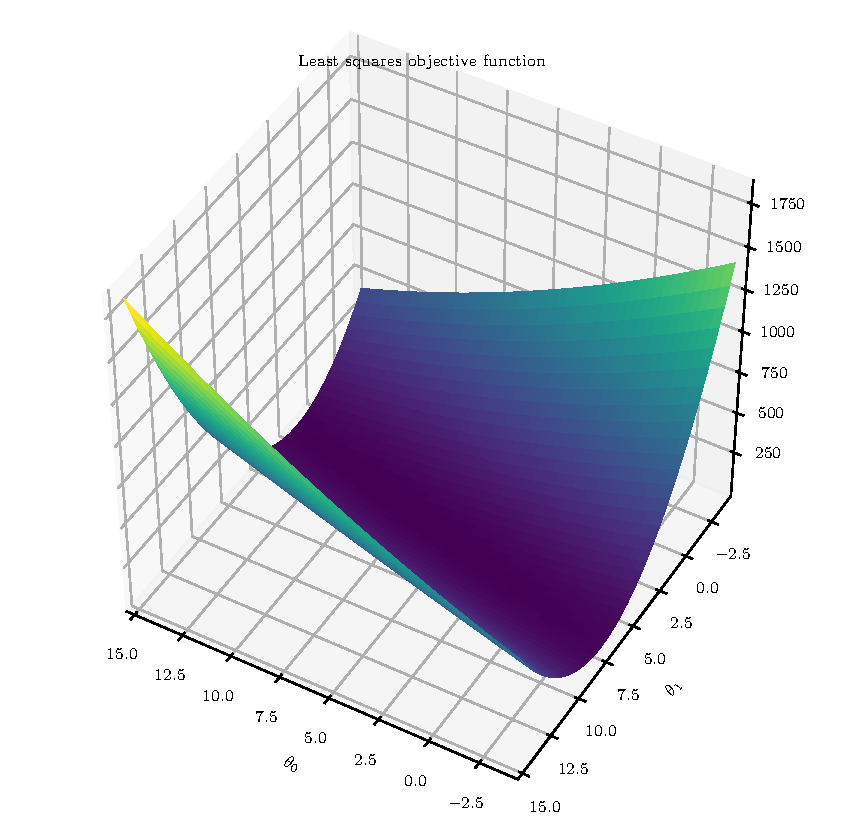
\includepdf[page=-]{ridge-gd.pdf}
%}

\end{document}
